\documentclass{article}

% Language setting
% Replace `english' with e.g. `spanish' to change the document language
\usepackage[english,russian]{babel}
\usepackage{amsmath}

%графика
\usepackage{wrapfig}
\usepackage{graphicx}
\usepackage{pgfplots}
\usepackage{tikz}


\usepackage{tcolorbox}

% Set page size and margins
% Replace `letterpaper' with `a4paper' for UK/EU standard size
\usepackage[letterpaper,top=2cm,bottom=2cm,left=3cm,right=3cm,marginparwidth=1.75cm]{geometry}

% Useful packages
\usepackage{amsmath}
\usepackage{amssymb}
\usepackage{graphicx}
\usepackage{fixltx2e}
\usepackage[colorlinks=true, allcolors=blue]{hyperref}

\usepackage{geometry}
\geometry{left=25mm,right=25mm,
 top=25mm,bottom=25mm}

\title{Web3: Defi \& NFT.\\
Lectures. Weeks 3-4. \\
Technical analysis. Технический анализ.}
\author{Yury Kulev}

% Колонтитулы
\usepackage{fancyhdr}
\pagestyle{fancy}
\renewcommand{\headrulewidth}{0.1mm}
\renewcommand{\footrulewidth}{0.1mm}
\lfoot{}
\rfoot{\thepage}
\cfoot{}
\rhead{CMF-2022}
\chead{}

\begin{document}
\maketitle

% Оглавление
\setcounter{tocdepth}{1} % {2} - в оглавлении участвуют chapter, section и subsection. {1} - только chapter и section
\renewcommand\contentsname{Contents}
\tableofcontents
\newpage

\renewcommand{\labelitemi}{\tiny$\bullet$}

 \section{Принципы технического анализа, его приложения и основные предположения}
 \begin{itemize}
     \item \textbf{Технический анализ} - это набор методов, используемый для анализа и построения прогноза цен финансовых инструментов с использованием графиков.

     \item Основой технического анализа является предположение, что рынки двигаются по определенным законам, которые имеют тенденцию повторяться со временем.

     \item Предполагается, что рынок отражает предполагаемые равновесные цены, соответствующие спросу и предложению.
 \end{itemize}


\section{Разные типы графиков технического анализа}
\begin{itemize}
    \item Линейчатая диаграмма (line chart) - по горизонтальной оси берутся даты, по вертикальной оси, обычно, цены закрытия периода.
    \begin{figure}[h]
    \centering
    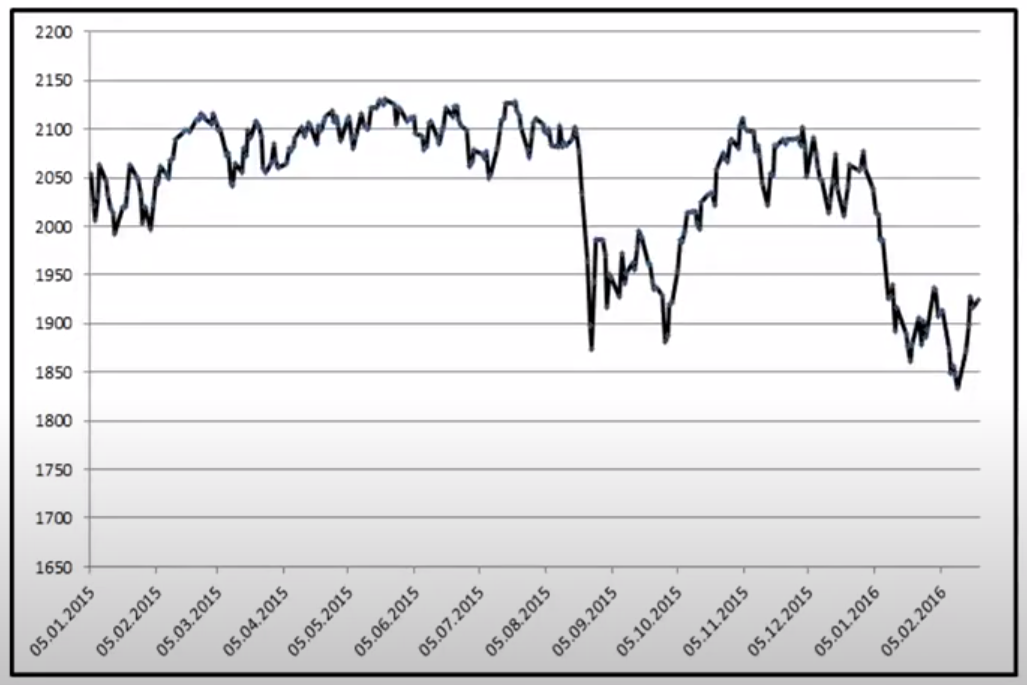
\includegraphics[width=0.57\textwidth]{line chart.png}
    \label{loadings}
    \end{figure}

    \item Японские свечи (candlestick chart) отображают информацию о поведении цены в выбранном таймфрейме. Тело свечи показывает цены открытия и закрытия дня, хвостики - максимум и минимум. Цвет свечи показывает как распологаются открытие/закрытие.
    \begin{figure}[h]
    \centering
    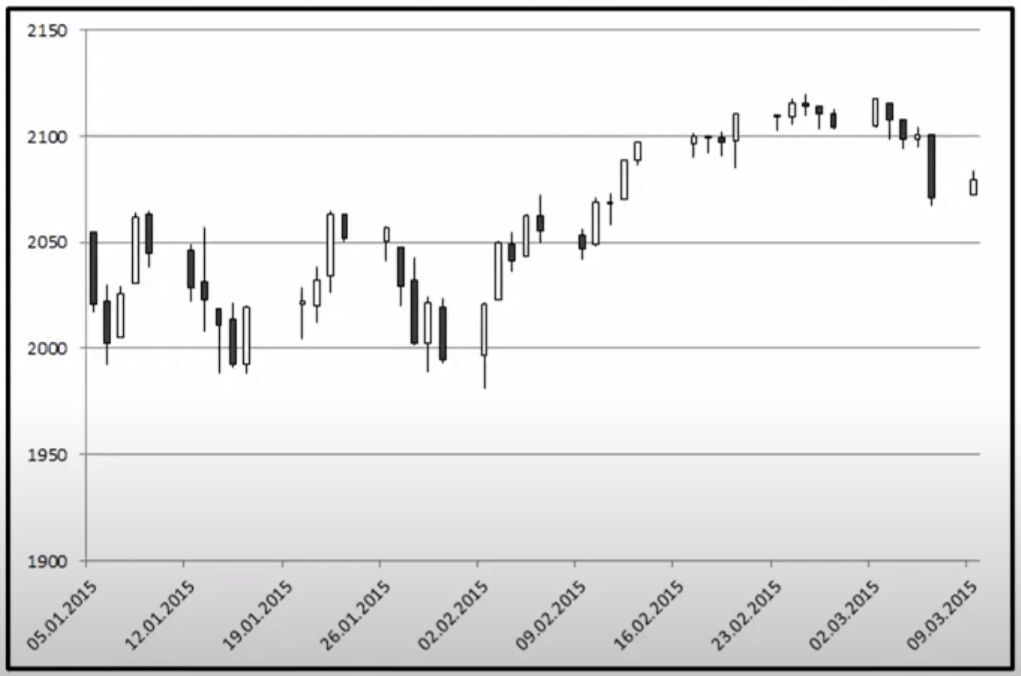
\includegraphics[width=0.57\textwidth]{candlestick chart.png}
    \label{loadings}
    \end{figure}

    \item Диаграмма объемов (volume charts) показывает в некоторых условных единицах объемы сделок, проводимых на соответствующем таймфрейме.
    \begin{figure}[h]
    \centering
    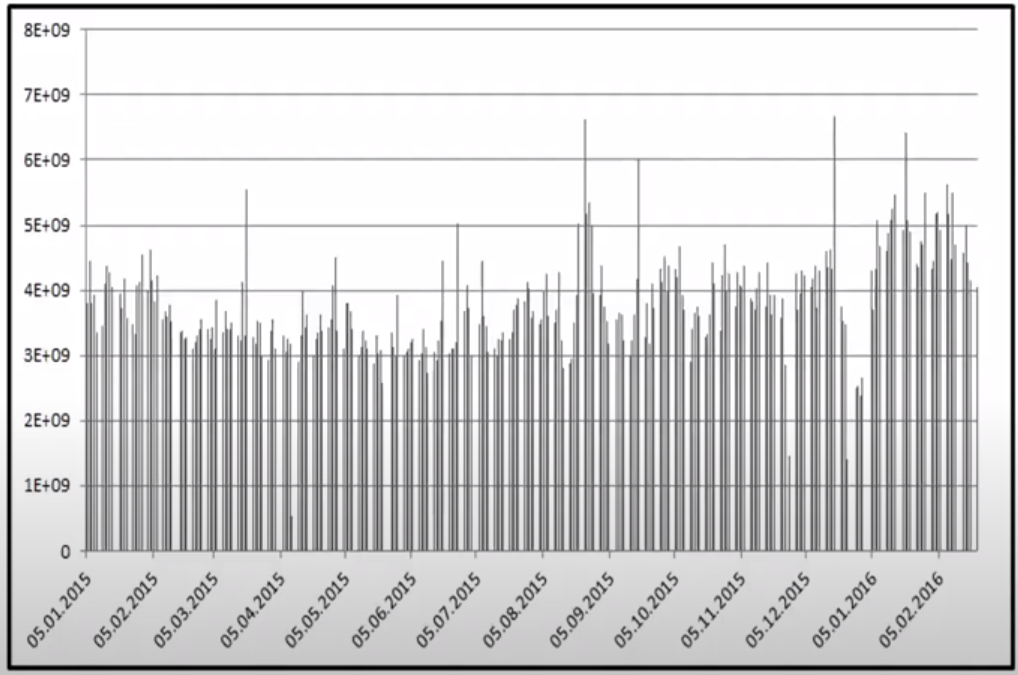
\includegraphics[width=0.57\textwidth]{volume chart.png}
    \label{loadings}
    \end{figure}
\end{itemize}

\section{Инструменты технического анализа}
\begin{itemize}
    \item \textbf{Линия поддержки (support line)} - прямая, такая что цена всегда остается выше этой прямой, обычно проводится через локальные минимумы цены.

    \item \textbf{Линия сопротивления (resistance line)} - верхняя граница цены, обычно проводится через локальные максимумы цены.

    \item \textbf{Изменение полярности (change in polarity)} - если цена пробивает линию поддержки/сопротивления, то та становится линией сопротивления/поддержки.
\end{itemize}
Инструменты технического анализа носят вероятностный характер.\\\\
\textbf{Линия тренда (trendline)} - некоторая средняя линия, которая отображает общую тенденцию рынка.
\begin{figure}[h]
\centering
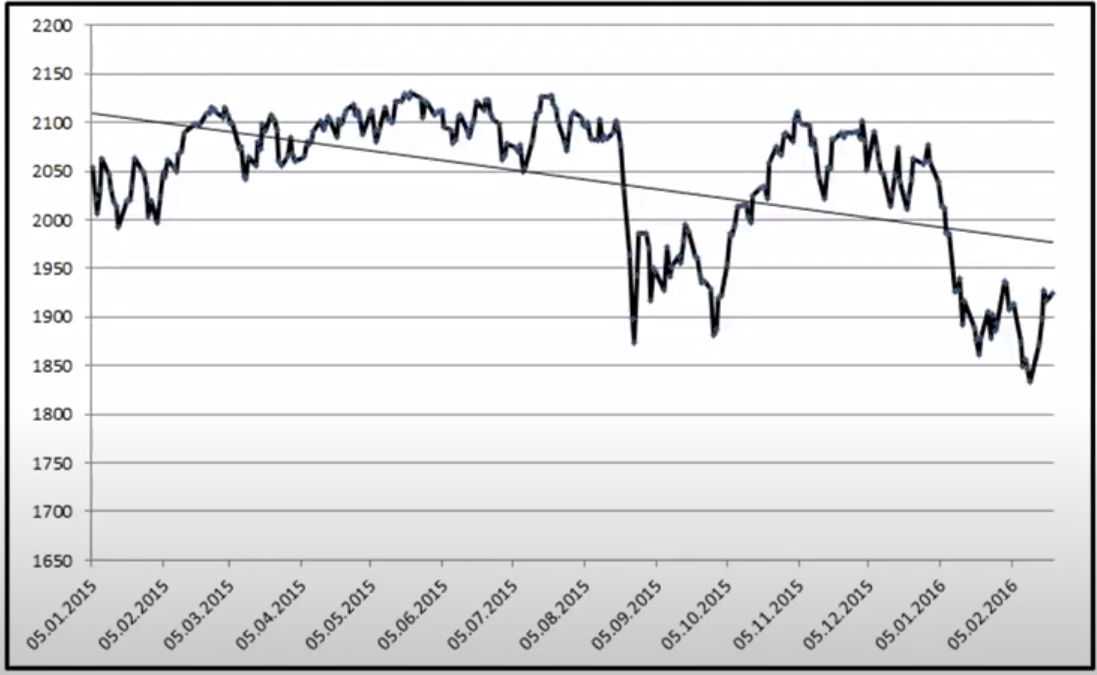
\includegraphics[width=0.57\textwidth]{trendline.png}
\label{loadings}
\end{figure}

\newpage
\section{Паттерны}
Паттерны - фигуры, которые предсказывают дальнейшее движение цены.
\begin{itemize}
    \item \textbf{Развороты (reversal patterns - RP)} - паттерны, которые сигнализируют об изменении тренда.

    \item \textbf{Паттерны продолжения (continuation patterns - CP)} - паттерны, которые говорят о том, что тренд будет продолжен.
\end{itemize}
Классическим примером RP является паттерн голова-плечи (neck-and-shoulders)\\
\begin{figure}[h]
\centering
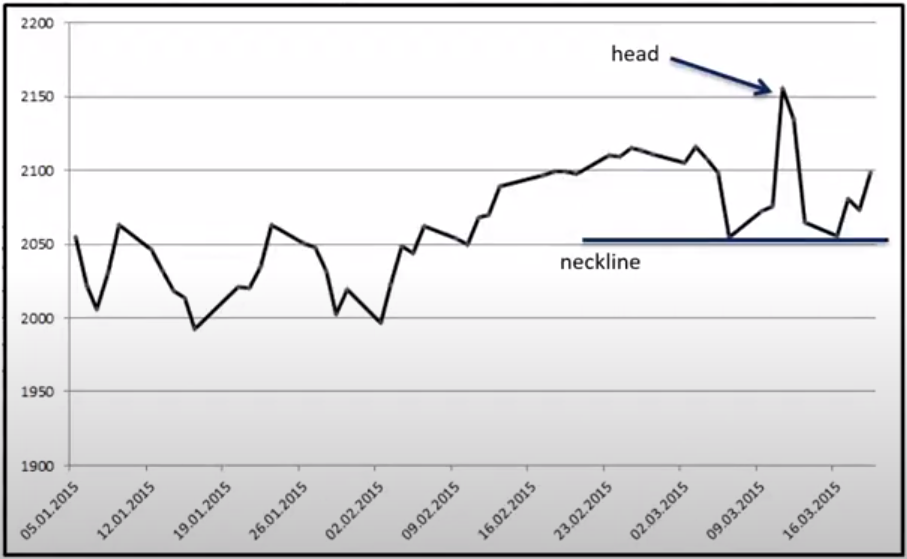
\includegraphics[width=0.57\textwidth]{patterns.png}
\label{loadings}
\end{figure}
\\Другие частые паттерны:
\begin{itemize}
    \item (RP) двойные/тройные вершины
    \item (RP) двойное/тройное дно
    \item (CP) треугольники
    \item (CP) прямоугольники
\end{itemize}

\section{Индикаторы}
Кроме паттернов, в техническом анализе используются индикаторы - это некоторые показатели, которые прогнозируют дальнейшее движение цены.
\begin{itemize}
    \item \textbf{Ценовые индикаторы (price-based indicators)}
    \begin{itemize}
        \item Скользящее среднее (moving average - MA) - это средняя цена за предыдущие $n$ шагов.
        \item Граница Боллинджера (Bollinger bands) - мы можем отступить от линии скользящего среднего вверх и вниз на $k$ среднеквадратичных отклонений цены (отложить вверх и вниз $k$ значений волатильности) - таким образом, получится коридор, в котором цена располагается с достаточно высокой вероятностью.
    \end{itemize}
    \item \textbf{Осцилляторы (oscillators)} - индикаторы, которые лучше всего работают, когда актив находится во флэте (нет ярко выраженного тренда).
    \begin{itemize}
        \item Индекс относительной силы (relative strength index - RSI) - низкие значения (близкие к нулю) означают, что инструмент перепродан, т.е. должно начаться движение вверх. Высокие значения (близкие к $100\%$) показывают, что инструмент перекуплен и должно начаться движение вниз.
        \item Скорость изменения (rate of change) - разница между ценой в момент $n$ и ценой в момент $n - k$.
    \end{itemize}
    \item \textbf{Неценовые индикторы (non-price-based indicators)}
    \begin{itemize}
        \item Любой индикатор настроения рынка
        \item Индекс волатильности (volatility index - VIX)
        \item Short interest ratio
        \item Mutual fund cash position
    \end{itemize}
\end{itemize}
\section{Технический анализ и циклы}
Технический анализ базируется на предположении, что ценовые паттерны имеют свойство повторяться. Часто ставят задачу выделения циклов для того, чтобы осуществлять прогноз не только цены, но и времени ее достижения.\\\\
Цикл Кондратьева (Kondratieff cycle) - 54 года.
\section{Волновая теория Эллиотта}
\textbf{Волновая теория Эллиотта (Elliot wave theory)} - тренд может быть разложен в пять волн по тренду и три коррекционные.\\\\
Считается, что все коррекционные волны идут в соответствии с числами Фибоначчи.
\section{Межрыночный анализ}
\textbf{Межрыночный/корреляционный анализ (intermarket analysis)} учитывает информацию о нескольких рынках одновременно.\\\\
Анализируя несколько рынков, исследователь может понять, какой рынок в настоящее время является опережающим/должен стать опережающим и проинвестировать соответствующим образом.
\end{document}

